\documentclass[12pt]{scrartcl}
\usepackage[hagavi]{azzam}

% Excircle - Solusi
% Pembahasan 16 soal Latihan: 3 Garis Bagi Luar, 3 Lemma Incenter-Excenter,
% 4 Jari-Jari dan Homoteti, 6 Esai Pilihan.
% Gaya penulisan mengikuti mo_material.md: solusi menumpuk persamaan ke bawah,
% satu langkah logis satu paragraf; semua gambar TikZ inline.
% Setiap jawaban numerik diverifikasi independen
% (lihat /tmp/verify_excircle.py).

\title{Excircle - Solusi}
\date{20 November 2026}

\begin{document}
\maketitle

\renewcommand*\contentsname{Daftar Isi}
\tableofcontents

\newpage

\section{Solusi Soal Latihan}

Setiap pembahasan memakai \istilah{lingkaran singgung luar}{excircle},
excenter, dan \istilah{garis bagi luar}{external angle bisector} dari Modul,
dengan notasi baku $a = BC$, $b = CA$, $c = AB$, dan $s$ setengah keliling.

\subsection{Garis Bagi Luar dan Panjang Singgung}

\begin{enumerate}
	\item Misalkan $I$ incenter $ABC$.
	Segiempat $ADIF$ mempunyai dua sudut siku-siku di $D$ dan $F$, jadi
	\[ \angle DIF = 180^\circ - \angle BAC = 110^\circ. \]
	Titik $E$ pada busur mayor $DF$ lingkaran dalam, sehingga sudut keliling
	\[ \angle DEF = \frac12 \angle DIF = 55^\circ. \]
	\begin{center}
	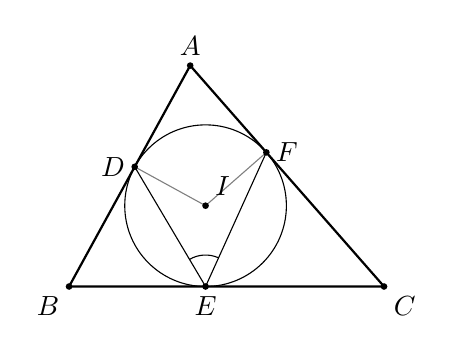
\begin{tikzpicture}[scale=0.8]
	    \coordinate (A) at (1.923,3.507);
	    \coordinate (B) at (0,0);
	    \coordinate (C) at (5,0);
	    \coordinate (I) at (2.167,1.283);
	    \coordinate (D) at (1.042,1.900);
	    \coordinate (E) at (2.167,0);
	    \coordinate (F) at (3.132,2.129);
	    \draw[thick] (A) -- (B) -- (C) -- cycle;
	    \draw (I) circle (1.283);
	    \draw[gray] (I) -- (D);
	    \draw[gray] (I) -- (F);
	    \draw (E) -- (D);
	    \draw (E) -- (F);
	    \draw (E) ++(66:0.5) arc (66:121:0.5);
	    \fill (A) circle (1.5pt);
	    \fill (B) circle (1.5pt);
	    \fill (C) circle (1.5pt);
	    \fill (I) circle (1.5pt);
	    \fill (D) circle (1.5pt);
	    \fill (E) circle (1.5pt);
	    \fill (F) circle (1.5pt);
	    \node[above] at (A) {$A$};
	    \node[below left] at (B) {$B$};
	    \node[below right] at (C) {$C$};
	    \node[above right] at (I) {$I$};
	    \node[left] at (D) {$D$};
	    \node[below] at (E) {$E$};
	    \node[right] at (F) {$F$};
	\end{tikzpicture}
	\end{center}

	\item Menurut teorema garis bagi luar,
	\[ \frac{PA}{PB} = \frac{CA}{CB} = \frac{3}{4}. \]
	Karena $A$ di antara $P$ dan $B$, tulis $PB = PA + AB$:
	\[ PA = \frac34(PA + AB), \]
	yaitu $PA = 3AB$. Jadi $PA:AB = 3:1$.
	\begin{center}
	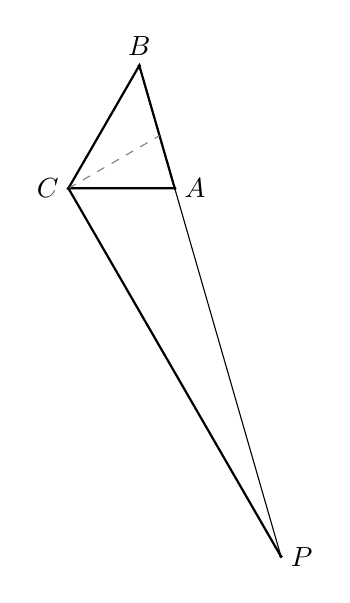
\begin{tikzpicture}[scale=0.45]
	    \coordinate (A) at (3,0);
	    \coordinate (B) at (2,3.464);
	    \coordinate (C) at (0,0);
	    \coordinate (P) at (6,-10.392);
	    \coordinate (E) at (2.571,1.485);
	    \draw[thick] (A) -- (B) -- (C) -- cycle;
	    \draw (B) -- (P);
	    \draw[thick] (C) -- (P);
	    \draw[gray,dashed] (C) -- (E);
	    \fill (A) circle (1.5pt);
	    \fill (B) circle (1.5pt);
	    \fill (C) circle (1.5pt);
	    \fill (P) circle (1.5pt);
	    \node[right] at (A) {$A$};
	    \node[above] at (B) {$B$};
	    \node[left] at (C) {$C$};
	    \node[right] at (P) {$P$};
	\end{tikzpicture}
	\end{center}

	\item Garis bagi dalam dan luar saling tegak lurus,
	jadi $\angle PAQ = 90^\circ$ dan $PQ$ diameter lingkaran $APQ$.
	Dari teorema garis bagi (dalam dan luar),
	\[ \frac{BP}{PC} = \frac{AB}{AC} = \frac{2}{1}, \qquad
	\frac{QB}{QC} = \frac{AB}{AC} = \frac{2}{1}. \]
	Dengan $BC = 240$ didapat $BP = 160$ dan ($Q$ di luar segmen)
	$QC = 240$, $QB = 480$. Maka
	\[ PQ = QB - PB = 480 - 160 = 320, \]
	jadi jari-jarinya $320/2 = 160$.
	\begin{center}
	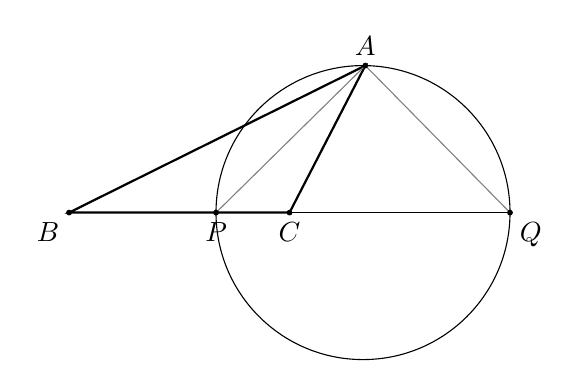
\begin{tikzpicture}[scale=0.7]
	    \coordinate (A) at (5.375,2.667);
	    \coordinate (B) at (0,0);
	    \coordinate (C) at (4,0);
	    \coordinate (P) at (2.667,0);
	    \coordinate (Q) at (8,0);
	    \coordinate (O) at (5.333,0);
	    \draw[thick] (A) -- (B) -- (C) -- cycle;
	    \draw (B) -- (Q);
	    \draw (O) circle (2.667);
	    \draw[gray] (A) -- (P);
	    \draw[gray] (A) -- (Q);
	    \fill (A) circle (1.5pt);
	    \fill (B) circle (1.5pt);
	    \fill (C) circle (1.5pt);
	    \fill (P) circle (1.5pt);
	    \fill (Q) circle (1.5pt);
	    \node[above] at (A) {$A$};
	    \node[below left] at (B) {$B$};
	    \node[below] at (C) {$C$};
	    \node[below] at (P) {$P$};
	    \node[below right] at (Q) {$Q$};
	\end{tikzpicture}
	\end{center}

\end{enumerate}

\subsection{Lemma Incenter-Excenter}

\begin{enumerate}[resume]
	\item Karena $D$ pada garis bagi $A$,
	$D$ titik tengah busur $BC$, jadi $DB = DI$ menurut lemma.
	\begin{enumerate}[(a)]
		\item Dari segitiga siku-siku di titik singgung,
		\[ AI = \frac{r}{\sin(A/2)}. \]
		Tali busur $DB$ menghadap sudut $A/2$ di $A$, jadi
		\[ DB = 2R\sin(A/2). \]
		Kesamaan $AI = DB$ setara dengan
		\[ r = 2R\sin^2(A/2) = R(1 - \cos A). \]
		Sekarang $1 - \cos A = 2(s-b)(s-c)/(bc)$,
		sementara $R = abc/(4\Delta)$ dan $r = \Delta/s$.
		Substitusi memberi
		\[ \frac{\Delta}{s}
		= \frac{abc}{4\Delta} \cdot \frac{2(s-b)(s-c)}{bc}, \]
		yaitu $2\Delta^2 = as(s-b)(s-c)$.
		Dengan Heron $\Delta^2 = s(s-a)(s-b)(s-c)$,
		ini setara $2(s-a) = a$, yaitu $2a = b + c$.
		Syarat terpenuhi, jadi $AI = DB = DI$:
		$I$ titik tengah $AD$.
		\item Karena $OA = OD$ (jari-jari) dan $I$ titik tengah $AD$,
		garis $OI$ adalah sumbu tegak lurus $AD$.
		Jadi $OI \perp AI$.
	\end{enumerate}
	\begin{center}
	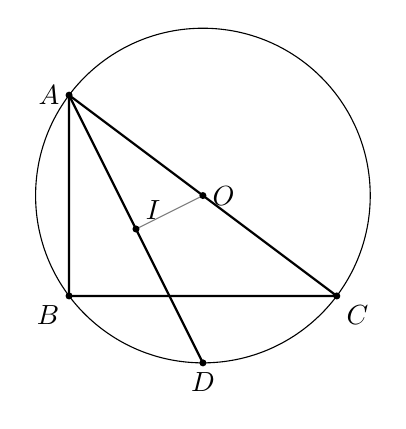
\begin{tikzpicture}[scale=0.85]
	    \coordinate (A) at (0,3);
	    \coordinate (B) at (0,0);
	    \coordinate (C) at (4,0);
	    \coordinate (I) at (1,1);
	    \coordinate (D) at (2,-1);
	    \coordinate (O) at (2,1.5);
	    \draw (O) circle (2.5);
	    \draw[thick] (A) -- (B) -- (C) -- cycle;
	    \draw[thick] (A) -- (D);
	    \draw[gray] (O) -- (I);
	    \fill (A) circle (1.5pt);
	    \fill (B) circle (1.5pt);
	    \fill (C) circle (1.5pt);
	    \fill (I) circle (1.5pt);
	    \fill (D) circle (1.5pt);
	    \fill (O) circle (1.5pt);
	    \node[left] at (A) {$A$};
	    \node[below left] at (B) {$B$};
	    \node[below right] at (C) {$C$};
	    \node[above right] at (I) {$I$};
	    \node[below] at (D) {$D$};
	    \node[right] at (O) {$O$};
	\end{tikzpicture}
	\end{center}

	\item Tulis $\omega$ untuk lingkaran $ADF$
	dan $X$ untuk perpotongan kedua garis $DN$ dengan $\omega$.
	Asumsikan posisi umum ($I$, $J$, $H$ terdefinisi
	dan segitiga $AHF$ takdegenerat).
	\begin{claim}
	$DI = DJ$, garis $DN$ melalui pusat $\omega$,
	dan $DX$ diameter $\omega$.
	\end{claim}
	Tali busur $DI$ menghadap $\angle DAI$ dan $DJ$ menghadap $\angle DAJ$,
	yang bernilai $90^\circ - \alpha/2$ dan $90^\circ + \alpha/2$
	dalam urutan tertentu ($\alpha = \angle CAB$,
	karena $AD$ garis bagi luar).
	Kedua sinusnya sama, jadi $DI = DJ$.
	Titik $N$ tengah-tengah $IJ$, jadi $DN$ sumbu tegak lurus $IJ$,
	yang selalu melalui pusat lingkaran.
	Akibatnya $DX$ diameter.
	\begin{claim}
	$X$, $A$, $E$ segaris dan $FX$ tegak lurus $BC$.
	\end{claim}
	Sudut $\angle XAD$ menghadap diameter, jadi $90^\circ$;
	sudut $\angle EAD$ juga $90^\circ$ (garis bagi dalam dan luar).
	Keduanya siku-siku di $A$ pada garis $AD$ yang sama,
	jadi $X$, $A$, $E$ segaris.
	Karena $F \in \omega$, sudut $\angle XFD$ menghadap diameter $DX$,
	jadi $90^\circ$; $D$ dan $F$ keduanya pada $BC$, jadi $FX \perp BC$.
	Dari dua klaim didapat dua segiempat siklis:
	$XFEH$ (sudut siku-siku di $H$ dan $F$)
	dan $ADEH$ (sudut siku-siku di $A$ dan $H$).
	Chase sudut berarah memberi ketiga garis bagi:
	\begin{align*}
	\angle HAE &= \angle HDE = \angle XDF = \angle XAF = \angle EAF, \\
	\angle AHE &= \angle ADE = \angle ADF = \angle AXF
	= \angle EXF = \angle EHF, \\
	\angle AFE &= \angle AFD = \angle AXD = \angle EXD
	= \angle EXH = \angle EFH,
	\end{align*}
	dengan tiap langkah memakai siklis $ADEH$, $\omega$, atau $XFEH$,
	atau kesegarisan $X$-$A$-$E$, $D$-$H$-$N$-$X$,
	dan $B$-$C$-$D$-$E$-$F$.
	Jadi $E$ terletak pada ketiga garis bagi sudut $AHF$.
	Karena $E$ di antara $D$ dan $F$, titik $E$ jatuh di dalam segitiga
	$AHF$ (bukan di luar), jadi $E$ incenter, bukan excenter.
	\begin{center}
	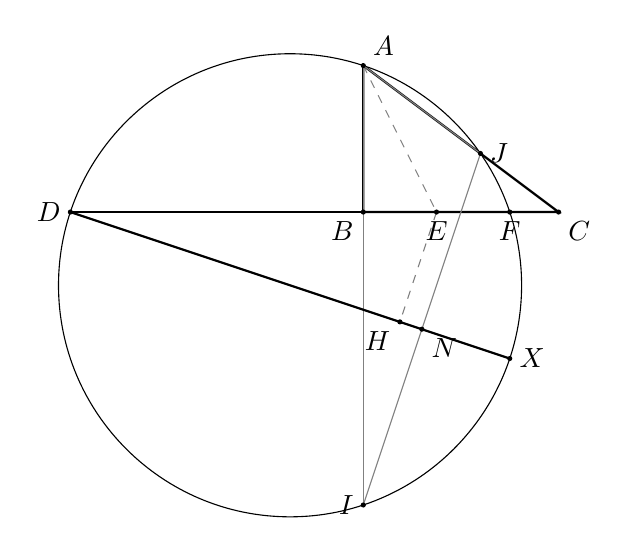
\begin{tikzpicture}[scale=0.62]
	    \coordinate (A) at (0,3);
	    \coordinate (B) at (0,0);
	    \coordinate (C) at (4,0);
	    \coordinate (D) at (-6,0);
	    \coordinate (E) at (1.5,0);
	    \coordinate (F) at (3,0);
	    \coordinate (O) at (-1.5,-1.5);
	    \coordinate (I) at (0,-6);
	    \coordinate (J) at (2.4,1.2);
	    \coordinate (N) at (1.2,-2.4);
	    \coordinate (H) at (0.75,-2.25);
	    \coordinate (X) at (3,-3);
	    \draw[thick] (A) -- (B) -- (C) -- cycle;
	    \draw (B) -- (D);
	    \draw (O) circle (4.743);
	    \draw[gray] (A) -- (I);
	    \draw[gray] (A) -- (J);
	    \draw[gray] (I) -- (J);
	    \draw[thick] (D) -- (X);
	    \draw[gray,dashed] (E) -- (H);
	    \draw[gray,dashed] (A) -- (E);
	    \fill (A) circle (1.5pt);
	    \fill (B) circle (1.5pt);
	    \fill (C) circle (1.5pt);
	    \fill (D) circle (1.5pt);
	    \fill (E) circle (1.5pt);
	    \fill (F) circle (1.5pt);
	    \fill (I) circle (1.5pt);
	    \fill (J) circle (1.5pt);
	    \fill (N) circle (1.5pt);
	    \fill (H) circle (1.5pt);
	    \fill (X) circle (1.5pt);
	    \node[above right] at (A) {$A$};
	    \node[below left] at (B) {$B$};
	    \node[below right] at (C) {$C$};
	    \node[left] at (D) {$D$};
	    \node[below] at (E) {$E$};
	    \node[below] at (F) {$F$};
	    \node[left] at (I) {$I$};
	    \node[right] at (J) {$J$};
	    \node[below right] at (N) {$N$};
	    \node[below left] at (H) {$H$};
	    \node[right] at (X) {$X$};
	\end{tikzpicture}
	\end{center}

	\item Bukti ini analitik memakai koordinat trilinear:
	perbandingan (bertanda) jarak ke $BC$, $CA$, $AB$.
	Garis bagi $BI$ adalah $\alpha = \gamma$,
	dan lingkaran umum berbentuk
	\[ a\beta\gamma + b\gamma\alpha + c\alpha\beta
	+ (u'\alpha + v'\beta + w'\gamma)(a\alpha + b\beta + c\gamma) = 0. \]
	Power $A$ terhadap $\Gamma$ memberi $AD \cdot AB = AE \cdot AC$.
	Bersama $AD + AE = a$ didapat
	\[ AD = \frac{ab}{b+c}, \qquad AE = \frac{ac}{b+c}. \]
	Melalui $B = (0:1:0)$ dan $C = (0:0:1)$ didapat $v' = w' = 0$,
	dan melalui $D$ (cek: $E$ memberi nilai sama) didapat
	\[ \Gamma: a\beta\gamma + b\gamma\alpha + c\alpha\beta
	- \frac{a}{b+c}\,\alpha(a\alpha + b\beta + c\gamma) = 0. \]
	Garis $BI$ berparametri $(t:1+t:t)$;
	substitusi ke $\Gamma$ memberi (selain $t = 0$, yaitu $B$)
	\[ t = -\frac{c}{\,b+c-a\,}, \qquad
	P = (-c:b-a:-c). \]
	Simetrisnya $Q = (-b:-b:c-a)$.
	Lingkaran melalui $A = (1:0:0)$ dan $I = (1:1:1)$ berbentuk
	\[ a\beta\gamma + b\gamma\alpha + c\alpha\beta
	+ (v''\beta + w''\gamma)(a\alpha + b\beta + c\gamma) = 0 \]
	dengan $v'' + w'' = -1$.
	Melalui $P$ memberi $v'' = -c/(b+c)$ dan $w'' = -b/(b+c)$.
	Substitusi $Q$ memberi pembilang
	\[ 2(s-c)(b+c) - ab - b^2 + c^2 - ac = 0, \]
	jadi $Q$ terletak pada lingkaran $AIP$.
	Terbukti $A$, $I$, $P$, $Q$ konsiklis.
	\begin{center}
	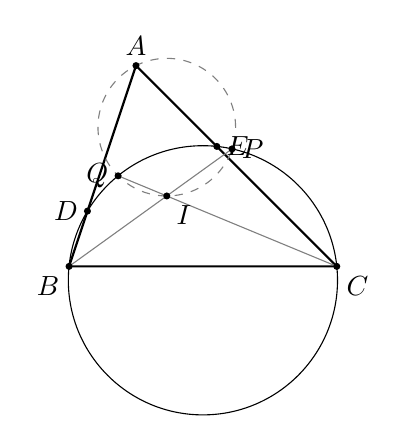
\begin{tikzpicture}[scale=0.85]
	    \coordinate (A) at (1,3);
	    \coordinate (B) at (0,0);
	    \coordinate (C) at (4,0);
	    \coordinate (D) at (0.275,0.826);
	    \coordinate (E) at (2.208,1.792);
	    \coordinate (I) at (1.460,1.052);
	    \coordinate (P) at (2.435,1.755);
	    \coordinate (Q) at (0.733,1.353);
	    \coordinate (O) at (2,-0.208);
	    \coordinate (O2) at (1.460,2.080);
	    \draw[thick] (A) -- (B) -- (C) -- cycle;
	    \draw (O) circle (2.011);
	    \draw[gray,dashed] (O2) circle (1.028);
	    \draw[gray] (B) -- (P);
	    \draw[gray] (C) -- (Q);
	    \fill (A) circle (1.5pt);
	    \fill (B) circle (1.5pt);
	    \fill (C) circle (1.5pt);
	    \fill (D) circle (1.5pt);
	    \fill (E) circle (1.5pt);
	    \fill (I) circle (1.5pt);
	    \fill (P) circle (1.5pt);
	    \fill (Q) circle (1.5pt);
	    \node[above] at (A) {$A$};
	    \node[below left] at (B) {$B$};
	    \node[below right] at (C) {$C$};
	    \node[left] at (D) {$D$};
	    \node[right] at (E) {$E$};
	    \node[below right] at (I) {$I$};
	    \node[right] at (P) {$P$};
	    \node[left] at (Q) {$Q$};
	\end{tikzpicture}
	\end{center}

\end{enumerate}

\subsection{Jari-Jari dan Homoteti}

\begin{enumerate}[resume]
	\item Dari $r = \Delta/s$ dan $r_a = \Delta/(s-a)$ (dan siklis),
	\[ r r_a r_b r_c
	= \frac{\Delta^4}{s(s-a)(s-b)(s-c)}
	= \frac{\Delta^4}{\Delta^2} = \Delta^2. \]
	Jadi $\Delta^2 = 1 \cdot 2 \cdot 3 \cdot 6 = 36$ dan $\Delta = 6$.
	Dari $r = 1$ didapat $s = 6$, lalu
	\[ s - a = \frac{\Delta}{r_a} = 3, \quad
	s - b = 2, \quad s - c = 1, \]
	jadi $\{a, b, c\} = \{3, 4, 5\}$.
	Akhirnya
	\[ R = \frac{abc}{4\Delta} = \frac{60}{24} = \frac52. \]

	\item Bukti koordinat. Taruh $B = (0, 0)$, $C = (a, 0)$,
	$D = (s-c, 0)$, $M = (a/2, 0)$, $A = (u, v)$,
	$N = ((u+s-c)/2, v/2)$, dan $I_a = (s-c, -r_a)$.
	Jika $b = c$, semua absisnya $a/2$: segaris vertikal.
	Andaikan $b \ne c$. Kemiringan $I_aM$:
	\[ \frac{r_a}{a/2 - (s-c)} = \frac{2r_a}{c-b}. \]
	Kemiringan $MN$:
	\[ \frac{v}{u + s - c - a}. \]
	Kesamaan kedua kemiringan setara dengan
	\[ v(c-b) = 2r_a(u + s - c - a). \]
	Substitusi $v = 2\Delta/a$, $r_a = \Delta/(s-a)$,
	dan $au = (a^2+c^2-b^2)/2$ mengubah kedua ruas
	menjadi $(c-b)(s-a)$. Jadi $I_a$, $M$, $N$ segaris.
	\begin{center}
	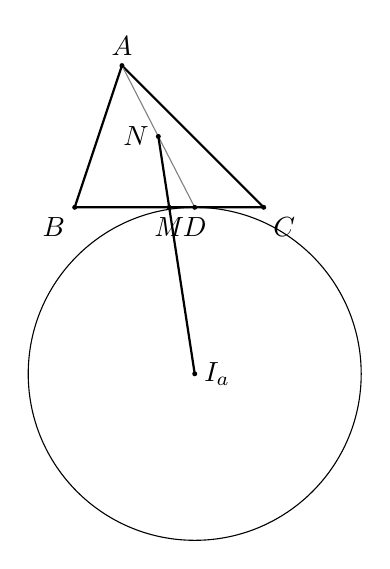
\begin{tikzpicture}[scale=0.6]
	    \coordinate (A) at (1,3);
	    \coordinate (B) at (0,0);
	    \coordinate (C) at (4,0);
	    \coordinate (D) at (2.540,0);
	    \coordinate (Ia) at (2.540,-3.524);
	    \coordinate (M) at (2,0);
	    \coordinate (N) at (1.770,1.5);
	    \draw[thick] (A) -- (B) -- (C) -- cycle;
	    \draw (Ia) circle (3.524);
	    \draw[gray] (A) -- (D);
	    \draw[thick] (Ia) -- (N);
	    \fill (A) circle (1.5pt);
	    \fill (B) circle (1.5pt);
	    \fill (C) circle (1.5pt);
	    \fill (D) circle (1.5pt);
	    \fill (Ia) circle (1.5pt);
	    \fill (M) circle (1.5pt);
	    \fill (N) circle (1.5pt);
	    \node[above] at (A) {$A$};
	    \node[below left] at (B) {$B$};
	    \node[below right] at (C) {$C$};
	    \node[below] at (D) {$D$};
	    \node[right] at (Ia) {$I_a$};
	    \node[below] at (M) {$M$};
	    \node[left] at (N) {$N$};
	\end{tikzpicture}
	\end{center}

	\item Taruh $C$ di titik asal; tulis vektor posisi $A$, $B$.
	Dari panjang garis singgung, $CK = s-a$ dan $CL = s-b$, jadi
	\[ K = \frac{s-a}{b}A, \qquad L = \frac{s-b}{a}B. \]
	Buktikan (b) dulu. Arah garisnya:
	\begin{align*}
	M_{KL} - M_{AB}
	&= \frac{K+L}{2} - \frac{A+B}{2} \\
	&= -\frac{s-c}{2}\left(\frac{A}{b} + \frac{B}{a}\right).
	\end{align*}
	Jumlah dua vektor satuan sepanjang $CA$ dan $CB$
	searah garis bagi $C$. Jadi garisnya sejajar garis bagi.
	Untuk (a): garis melalui titik tengah $AB$ yang sejajar garis bagi
	memotong sisi $CA$ atau $CB$ pada jarak $|a-b|/2$ dari $C$.
	Dari titik potong ke $A$ lalu ke titik tengah $AB$ berjarak
	$(a+b)/2 + c/2 = s$, dan sisi satunya sisanya. Terbukti.
	\begin{center}
	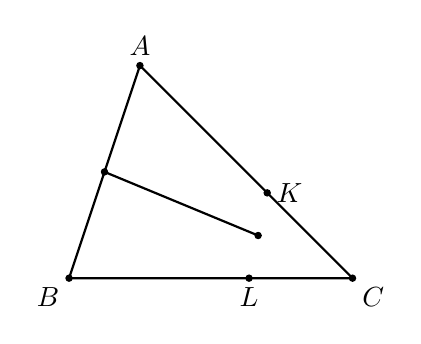
\begin{tikzpicture}[scale=0.9]
	    \coordinate (A) at (1,3);
	    \coordinate (B) at (0,0);
	    \coordinate (C) at (4,0);
	    \coordinate (K) at (2.796,1.204);
	    \coordinate (L) at (2.540,0);
	    \coordinate (Mkl) at (2.668,0.602);
	    \coordinate (Mab) at (0.5,1.5);
	    \draw[thick] (A) -- (B) -- (C) -- cycle;
	    \draw[thick] (Mkl) -- (Mab);
	    \fill (A) circle (1.5pt);
	    \fill (B) circle (1.5pt);
	    \fill (C) circle (1.5pt);
	    \fill (K) circle (1.5pt);
	    \fill (L) circle (1.5pt);
	    \fill (Mkl) circle (1.5pt);
	    \fill (Mab) circle (1.5pt);
	    \node[above] at (A) {$A$};
	    \node[below left] at (B) {$B$};
	    \node[below right] at (C) {$C$};
	    \node[right] at (K) {$K$};
	    \node[below] at (L) {$L$};
	\end{tikzpicture}
	\end{center}

	\item Misalkan $AB = AC = L$ dan alas $BC = m$.
	Taruh $M$ titik tengah $BC$ di titik asal:
	$B = (-m/2, 0)$, $C = (m/2, 0)$, $A = (0, h)$
	dengan $h^2 = L^2 - m^2/4$.
	Dengan $s = L + m/2$ dan $\Delta = mh/2$:
	\[ r = \frac{mh}{2s}, \quad
	r_a = \frac{mh}{2(s-m)}, \quad
	r_b = r_c = h. \]
	Tulis $u = s$, $v = s - m$; maka $h^2 = uv$.
	Incenter $I = (0, r)$ dan $I_a = (0, -r_a)$,
	jadi $II_a = r + r_a$.
	Singgung dalam memberi $\rho = r + 2r_a$ untuk jari-jari $\omega$
	(pilihan tanda satunya, $\rho = -r$, mustahil).
	Singgung luar dengan $B$-excircle memberi
	$\rho = II_b - r_b$, dengan $II_b^2 = L^2 + (h-r)^2$.
	Persamaan $(r + 2r_a + h)^2 = L^2 + (h-r)^2$ dijabarkan menjadi
	\[ r_a^2 + rr_a + rh + hr_a = \frac{L^2}{4}. \]
	Substitusi $r$, $r_a$, $h^2 = uv$ memberi
	\[ \frac{m^2u}{4v} + \frac{m^2}{4} + mL = \frac{L^2}{4}, \]
	yaitu $2m(m + 2v) = Lv$.
	Dengan $v = L - m/2$ ini menjadi $L^2 = 9mL/2$,
	jadi $L/m = 9/2$.
	Sisi bulat terkecil: $m = 2$, $L = 9$, keliling $20$.
	Contoh $(9, 9, 2)$ memenuhi segitiga dan kedua kesinggungan,
	jadi $20$ minimum.

\end{enumerate}

\subsection{Esai Pilihan}

\begin{enumerate}[resume]
	\item Bukti barycentric terhadap $ABC$.
	Titik tengah adalah rata-rata koordinat barycentric ternormalisasi,
	jadi dari $B_1 = (a:-b:c)$ dan $C_1 = (a:b:-c)$ didapat
	\[ D = (a^2:-b(b-c):c(b-c)). \]
	Garis $CD$ memotong $AB$ ($z = 0$) di $E = (a^2:b(c-b):0)$,
	dan garis $BD$ memotong $AC$ ($y = 0$) di $F = (a^2:0:c(b-c))$.
	Garis $EF$ memotong $BC$ ($x = 0$) di
	\[ G = (0:b:c). \]
	Karena $BG:GC = c:b = AB:AC$ dengan $G$ pada segmen $BC$,
	garis $AG$ membagi sudut $A$ (konvers teorema garis bagi).
	\begin{center}
	\begin{tikzpicture}[scale=0.42]
	    \coordinate (A) at (9,12);
	    \coordinate (B) at (0,0);
	    \coordinate (C) at (14,0);
	    \coordinate (B1) at (21,10.5);
	    \coordinate (C1) at (-7,14);
	    \coordinate (D) at (7,12.25);
	    \coordinate (E) at (7.946,10.595);
	    \coordinate (F) at (8.096,14.169);
	    \coordinate (G) at (7.5,0);
	    \draw[thick] (A) -- (B) -- (C) -- cycle;
	    \draw[gray,dashed] (B1) -- (C1);
	    \draw[gray] (C) -- (E);
	    \draw[gray] (B) -- (F);
	    \draw[gray] (E) -- (G);
	    \draw[thick] (A) -- (G);
	    \fill (A) circle (1.5pt);
	    \fill (B) circle (1.5pt);
	    \fill (C) circle (1.5pt);
	    \fill (B1) circle (1.5pt);
	    \fill (C1) circle (1.5pt);
	    \fill (D) circle (1.5pt);
	    \fill (E) circle (1.5pt);
	    \fill (F) circle (1.5pt);
	    \fill (G) circle (1.5pt);
	    \node[below left] at (A) {$A$};
	    \node[below left] at (B) {$B$};
	    \node[below right] at (C) {$C$};
	    \node[right] at (B1) {$B_1$};
	    \node[left] at (C1) {$C_1$};
	    \node[above] at (D) {$D$};
	    \node[right] at (E) {$E$};
	    \node[right] at (F) {$F$};
	    \node[below] at (G) {$G$};
	\end{tikzpicture}
	\end{center}

	\item Bukti barycentric. $D = (1:1:0)$ dan $J = (a:-b:c)$.
	\begin{enumerate}[(a)]
		\item Garis $DJ$ memotong $CA$ ($y = 0$) di
		\[ F = (a+b:0:c). \]
		Vektor $IF = F - I$ searah $(1:-1:0)$,
		yaitu arah $AB$. Jadi $IF \parallel AB$.
		\item Tulis $E = (0:\beta:\gamma)$ di $BC$.
		Garis melalui $E$ sejajar $AB$ (arah $(1:-1:0)$)
		memotong garis bagi $C$ ($x:y = a:b$) di
		\[ P = (a\beta:b\beta:(a+b)\gamma). \]
		Garis $AP$ dan $BJ$ berpotongan di
		\[ X = (a(a+b)\gamma:bc\beta:c(a+b)\gamma), \]
		yang juga memenuhi persamaan garis $EF$.
		Jadi $AP$, $BJ$, $EF$ berpotongan di $X$.
	\end{enumerate}
	\begin{center}
	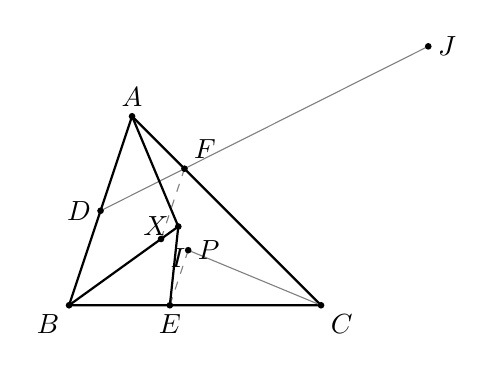
\begin{tikzpicture}[scale=0.8]
	    \coordinate (A) at (1,3);
	    \coordinate (B) at (0,0);
	    \coordinate (C) at (4,0);
	    \coordinate (I) at (1.460,1.052);
	    \coordinate (J) at (5.702,4.110);
	    \coordinate (D) at (0.5,1.5);
	    \coordinate (F) at (1.832,2.168);
	    \coordinate (E) at (1.6,0);
	    \coordinate (P) at (1.891,0.874);
	    \coordinate (X) at (1.734,1.250);
	    \draw[thick] (A) -- (B) -- (C) -- cycle;
	    \draw[gray] (D) -- (J);
	    \draw[gray,dashed] (I) -- (F);
	    \draw[gray,dashed] (E) -- (P);
	    \draw[gray] (C) -- (P);
	    \draw[thick] (A) -- (X);
	    \draw[thick] (B) -- (X);
	    \draw[thick] (E) -- (X);
	    \fill (A) circle (1.5pt);
	    \fill (B) circle (1.5pt);
	    \fill (C) circle (1.5pt);
	    \fill (I) circle (1.5pt);
	    \fill (J) circle (1.5pt);
	    \fill (D) circle (1.5pt);
	    \fill (F) circle (1.5pt);
	    \fill (E) circle (1.5pt);
	    \fill (P) circle (1.5pt);
	    \fill (X) circle (1.5pt);
	    \node[above] at (A) {$A$};
	    \node[below left] at (B) {$B$};
	    \node[below right] at (C) {$C$};
	    \node[below right] at (I) {$I$};
	    \node[right] at (J) {$J$};
	    \node[left] at (D) {$D$};
	    \node[above right] at (F) {$F$};
	    \node[below] at (E) {$E$};
	    \node[right] at (P) {$P$};
	    \node[left] at (X) {$X$};
	\end{tikzpicture}
	\end{center}

	\item Menurut contoh pengenalan konfigurasi di Modul,
	$D$ adalah titik singgung $A$-excircle.
	Taruh $D$ di titik asal dan $BC$ sebagai sumbu-$x$:
	$B = (-d_1, 0)$, $C = (d_2, 0)$ dengan $d_1 = s-c$, $d_2 = s-b$,
	dan $A = (p, q)$.
	Klaimnya: garis horizontal $y = r/2$ menyinggung kedua lingkaran.
	Dari $X \in AD$ dan power $D$ terhadap $(ABC)$,
	pusat $(BDX)$ adalah $(-d_1/2, y_1)$ dengan
	\[ y_1 = \frac{d_1(p-d_2)}{2q}, \]
	dan pusat $(CDX)$ adalah $(d_2/2, y_2)$ dengan
	\[ y_2 = -\frac{d_2(d_1+p)}{2q}. \]
	Garis $y = r/2$ menyinggung $(BDX)$ tepat saat
	$(d_1/2)^2 = r^2/4 - ry_1$.
	Substitusi $y_1$, $p = s(c-b)/a$, $r = aq/(2s)$,
	dan $r^2 = (s-a)(s-b)(s-c)/s$ (Heron)
	menyederhanakan kedua ruas menjadi
	$(s-c)(ab+sc-sa-sb)/s$.
	Untuk $(CDX)$, syarat $(d_2/2)^2 = r^2/4 - ry_2$
	setelah substitusi yang sama menjadi
	$s(s-b) = (s-a)(s-c) + a(s-c) + s(c-b)$,
	yaitu $s(s-b) = s(s-b)$.
	Jadi satu garis singgung persekutuan
	(atas atau melintang, bergantung konfigurasi) sejajar $BC$.
	\begin{center}
	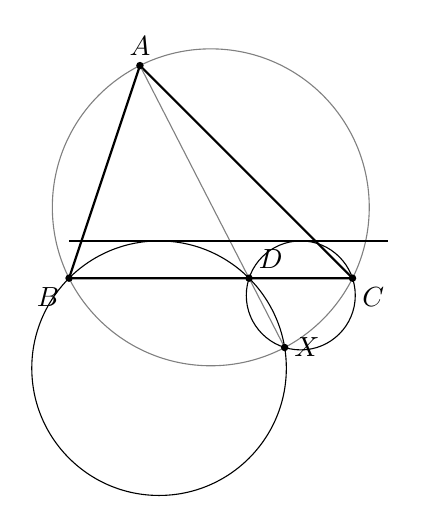
\begin{tikzpicture}[scale=0.9]
	    \coordinate (A) at (1,3);
	    \coordinate (B) at (0,0);
	    \coordinate (C) at (4,0);
	    \coordinate (D) at (2.540,0);
	    \coordinate (X) at (3.042,-0.978);
	    \coordinate (O1) at (1.270,-1.270);
	    \coordinate (O2) at (3.270,-0.243);
	    \coordinate (O) at (2,1);
	    \draw[thick] (A) -- (B) -- (C) -- cycle;
	    \draw[gray] (O) circle (2.236);
	    \draw[gray] (A) -- (X);
	    \draw (O1) circle (1.796);
	    \draw (O2) circle (0.769);
	    \draw[thick] (0,0.526) -- (4.5,0.526);
	    \fill (A) circle (1.5pt);
	    \fill (B) circle (1.5pt);
	    \fill (C) circle (1.5pt);
	    \fill (D) circle (1.5pt);
	    \fill (X) circle (1.5pt);
	    \node[above] at (A) {$A$};
	    \node[below left] at (B) {$B$};
	    \node[below right] at (C) {$C$};
	    \node[above right] at (D) {$D$};
	    \node[right] at (X) {$X$};
	\end{tikzpicture}
	\end{center}

	\item Bukti barycentric. Titik singgung:
	$M = (0:d_2:d_1)$ di $BC$ ($d_1 = s-c$, $d_2 = s-b$),
	$K = (-d_1:s:0)$ pada garis $AB$,
	$L = (-d_2:0:s)$ pada garis $AC$.
	Garis $LM$ adalah $sx - d_1y + d_2z = 0$
	dan garis $BJ$ ($J = (-a:b:c)$) adalah $cx + az = 0$,
	sehingga
	\[ F = (-ad_1:d_2c-sa:cd_1). \]
	Garis $AF$ memotong $BC$ di $S = (0:d_2c-sa:cd_1)$,
	dan simetrisnya $T = (0:bd_2:bd_1-sa)$.
	Jumlah koordinat $S$ adalah $-ad_1$ dan jumlah $T$ adalah $-ad_2$,
	jadi titik tengah ternormalisasinya berkoordinat-$y$
	\[ \frac12\left(\frac{sa-d_2c}{ad_1} - \frac{b}{a}\right)
	= \frac{sa-d_2c-bd_1}{2ad_1}. \]
	Nilai ini sama dengan $d_2/a$ (koordinat $M$),
	sebab $sa = d_2c+bd_1+2d_1d_2$:
	tulis $x = s-a$, $y = s-b$, $z = s-c$,
	maka ruas kanan $cy+bz+2yz = s(y+z) = sa$.
	Jadi $M$ titik tengah $ST$.
	\begin{center}
	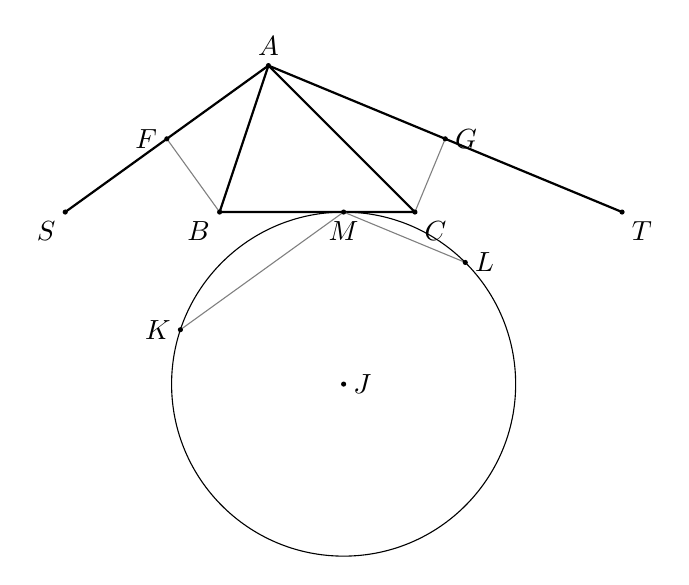
\begin{tikzpicture}[scale=0.62]
	    \coordinate (A) at (1,3);
	    \coordinate (B) at (0,0);
	    \coordinate (C) at (4,0);
	    \coordinate (J) at (2.540,-3.524);
	    \coordinate (M) at (2.540,0);
	    \coordinate (K) at (-0.803,-2.410);
	    \coordinate (L) at (5.032,-1.032);
	    \coordinate (F) at (-1.081,1.5);
	    \coordinate (G) at (4.621,1.5);
	    \coordinate (S) at (-3.162,0);
	    \coordinate (T) at (8.243,0);
	    \draw[thick] (A) -- (B) -- (C) -- cycle;
	    \draw (J) circle (3.524);
	    \draw[gray] (B) -- (F);
	    \draw[gray] (C) -- (G);
	    \draw[gray] (L) -- (M);
	    \draw[gray] (K) -- (M);
	    \draw[thick] (A) -- (S);
	    \draw[thick] (A) -- (T);
	    \fill (A) circle (1.5pt);
	    \fill (B) circle (1.5pt);
	    \fill (C) circle (1.5pt);
	    \fill (J) circle (1.5pt);
	    \fill (M) circle (1.5pt);
	    \fill (K) circle (1.5pt);
	    \fill (L) circle (1.5pt);
	    \fill (F) circle (1.5pt);
	    \fill (G) circle (1.5pt);
	    \fill (S) circle (1.5pt);
	    \fill (T) circle (1.5pt);
	    \node[above] at (A) {$A$};
	    \node[below left] at (B) {$B$};
	    \node[below right] at (C) {$C$};
	    \node[right] at (J) {$J$};
	    \node[below] at (M) {$M$};
	    \node[left] at (K) {$K$};
	    \node[right] at (L) {$L$};
	    \node[left] at (F) {$F$};
	    \node[right] at (G) {$G$};
	    \node[below left] at (S) {$S$};
	    \node[below right] at (T) {$T$};
	\end{tikzpicture}
	\end{center}

	\item Misalkan $M_b$, $M_c$, $M$ berturut-turut titik tengah
	$IB$, $IC$, $IJ$.
	Menurut lemma, $M$ titik tengah busur $BC$ sekaligus pusat
	lingkaran $BICJ$.
	Garis $M_bM$ sumbu tegak lurus talibusur $IB$ pada lingkaran $BIC$,
	sedangkan $O_bM_b$ sumbu tegak lurus talibusur yang sama pada
	$\omega_b$. Jadi $M$, $O_b$, $M_b$ segaris,
	dan simetrisnya $M$, $O_c$, $M_c$ segaris.
	Perhatikan $MO_b \perp BI$ dan $O_cI \perp BI$
	(jari-jari ke titik singgung $\omega_c$),
	jadi $MO_b \parallel O_cI$; simetrisnya $MO_c \parallel O_bI$.
	Akibatnya $MO_bIO_c$ jajar genjang,
	sehingga diagonal-diagonalnya saling membagi dua:
	\[ IK = \frac12 IM = \frac14 IJ. \]
	Jadi $IK/KJ = (1/4)/(3/4) = 1/3$.
	\begin{center}
	\begin{tikzpicture}[scale=2.5]
	    \tkzDefPoint(125:1){A}
	    \tkzDefPoint(210:1){B}
	    \tkzDefPoint(-30:1){C}
	    \tkzDefTriangleCenter[circum](A,B,C)\tkzGetPoint{O}
	    \tkzDrawCircle(O,A)
	    \tkzInCenter(A,B,C)\tkzGetPoint{I}
	    \tkzInterLC[common=A](A,I)(O,A)\tkzGetFirstPoint{M}
	    \tkzDefPointBy[symmetry=center M](I)\tkzGetPoint{J}
	    \tkzDefTriangleCenter[circum](B,I,C)\tkzGetPoint{Obic}
	    \tkzDrawCircle[blue](Obic,B)
	    \tkzDrawSegment(A,J)
	    \tkzDrawSegments[blue](B,I C,I)
	    \tkzDefMidPoint(I,B)\tkzGetPoint{Mb}
	    \tkzDefLine[orthogonal=through I](I,C)\tkzGetPoint{icp}
	    \tkzDefLine[orthogonal=through Mb](I,B)\tkzGetPoint{mbp}
	    \tkzInterLL(I,icp)(Mb,mbp)\tkzGetPoint{Ob}
	    \tkzDefMidPoint(I,C)\tkzGetPoint{Mc}
	    \tkzDefLine[orthogonal=through I](I,B)\tkzGetPoint{ibp}
	    \tkzDefLine[orthogonal=through Mc](I,C)\tkzGetPoint{mcp}
	    \tkzInterLL(I,ibp)(Mc,mcp)\tkzGetPoint{Oc}
	    \tkzDrawSegments[green!60!black](I,Ob Ob,M M,Oc Oc,I)
	    \tkzDrawSegment[green!60!black](Ob,Oc)
	    \tkzInterLL(I,M)(Ob,Oc)\tkzGetPoint{K}
	    \tkzDrawPoints[fill=black, size=3](A,B,C,I,M,J,Mb,Ob,Mc,Oc,K)
	    \tkzLabelPoint[above left](A){$A$}
	    \tkzLabelPoint[left](B){$B$}
	    \tkzLabelPoint[right](C){$C$}
	    \tkzLabelPoint[above right](I){$I$}
	    \tkzLabelPoint[below right](M){$M$}
	    \tkzLabelPoint[below](J){$J$}
	    \tkzLabelPoint[above left](Mb){$M_b$}
	    \tkzLabelPoint[above right](Ob){$O_b$}
	    \tkzLabelPoint[above right](Mc){$M_c$}
	    \tkzLabelPoint[below right](Oc){$O_c$}
	    \tkzLabelPoint[below left](K){$K$}
	\end{tikzpicture}
	\end{center}

	\item Tulis $T$ titik tengah $KM$.
	Karena $AK = AM = s$, segitiga $AKM$ samakaki dan $T$ terletak
	pada garis bagi $A$. Titik $T \ne A$ pada lingkaran luar,
	jadi $T$ adalah titik tengah busur $BC$.
	Dari segitiga samakaki, $AT = s\cos(A/2)$.
	Di sisi lain Ptolemy pada $ABTC$ memberi
	\[ AT = \frac{TB(b+c)}{a}
	= \frac{2R\sin(A/2)(b+c)}{a}
	= \frac{b+c}{2\cos(A/2)}. \]
	Persamaannya menjadi $s(1+\cos A) = b+c$,
	yaitu
	\[ \cos A = \frac{s-a}{s}. \]
	Taruh $B = (0,0)$, $C = (a,0)$:
	$O = (a/2, R\cos A)$, $I = (s-b, r)$, $N = (s-c, 0)$.
	Jika $b = c$, ketiganya pada sumbu simetri $x = a/2$.
	Andaikan $b \ne c$: segaris $O$, $I$, $N$ setara dengan
	\[ \frac{r - R\cos A}{(c-b)/2}
	= \frac{-R\cos A}{(b-c)/2}, \]
	yaitu $r = 2R\cos A$.
	Tulis $p = \sin(B/2)\sin(C/2)$ dan $q = \cos(B/2)\cos(C/2)$,
	jadi $q - p = \sin(A/2)$.
	Dengan $r = 4R\sin(A/2)\sin(B/2)\sin(C/2)$ dan
	$(s-a)/s = \tan(B/2)\tan(C/2)$
	(sebab $\tan(B/2)\tan(C/2) = r^2/((s-b)(s-c)) = (s-a)/s$),
	kondisi $\cos A = (s-a)/s$ adalah $\cos A = p/q$,
	sehingga
	\[ \frac{r}{2R\cos A}
	= \frac{2\sin(A/2) \cdot p}{p/q}
	= 2\sin\frac{A}{2} \cdot q. \]
	Dari $\cos A = p/q$ dan $q - p = \sin(A/2)$ didapat
	$q = 1/(2\sin(A/2))$,
	jadi ruas kanan $1$.
	Akibatnya $r = 2R\cos A$ dan $O$, $I$, $N$ segaris.
	\begin{center}
	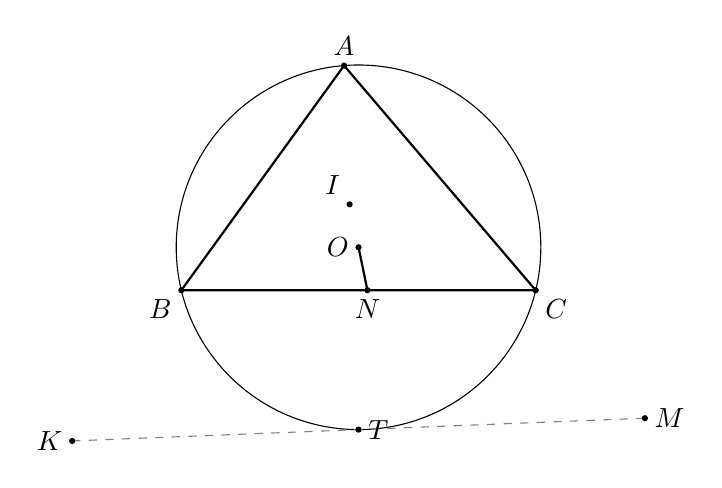
\begin{tikzpicture}[scale=0.75]
	    \coordinate (A) at (2.755,3.804);
	    \coordinate (B) at (0,0);
	    \coordinate (C) at (6,0);
	    \coordinate (N) at (3.151,0);
	    \coordinate (K) at (-1.849,-2.552);
	    \coordinate (M) at (7.849,-2.167);
	    \coordinate (T) at (3,-2.360);
	    \coordinate (O) at (3,0.727);
	    \coordinate (I) at (2.849,1.454);
	    \draw[thick] (A) -- (B) -- (C) -- cycle;
	    \draw (O) circle (3.087);
	    \draw[gray,dashed] (K) -- (M);
	    \draw[thick] (O) -- (N);
	    \fill (A) circle (1.5pt);
	    \fill (B) circle (1.5pt);
	    \fill (C) circle (1.5pt);
	    \fill (N) circle (1.5pt);
	    \fill (K) circle (1.5pt);
	    \fill (M) circle (1.5pt);
	    \fill (T) circle (1.5pt);
	    \fill (O) circle (1.5pt);
	    \fill (I) circle (1.5pt);
	    \node[above] at (A) {$A$};
	    \node[below left] at (B) {$B$};
	    \node[below right] at (C) {$C$};
	    \node[below] at (N) {$N$};
	    \node[left] at (K) {$K$};
	    \node[right] at (M) {$M$};
	    \node[right] at (T) {$T$};
	    \node[left] at (O) {$O$};
	    \node[above left] at (I) {$I$};
	\end{tikzpicture}
	\end{center}

\end{enumerate}

\end{document}
